\chapter{Processo di sviluppo}
\section{Sistemi di versionamento}
Il progetto è stato versionato con \textbf{Git}, utilizzando un flusso di lavoro semplice e chiaro per garantire tracciabilità e qualità.

Di seguito è riportato il grafico dei commit giornalieri nel periodo di sviluppo considerato.

\begin{figure}[h]
	\centering
	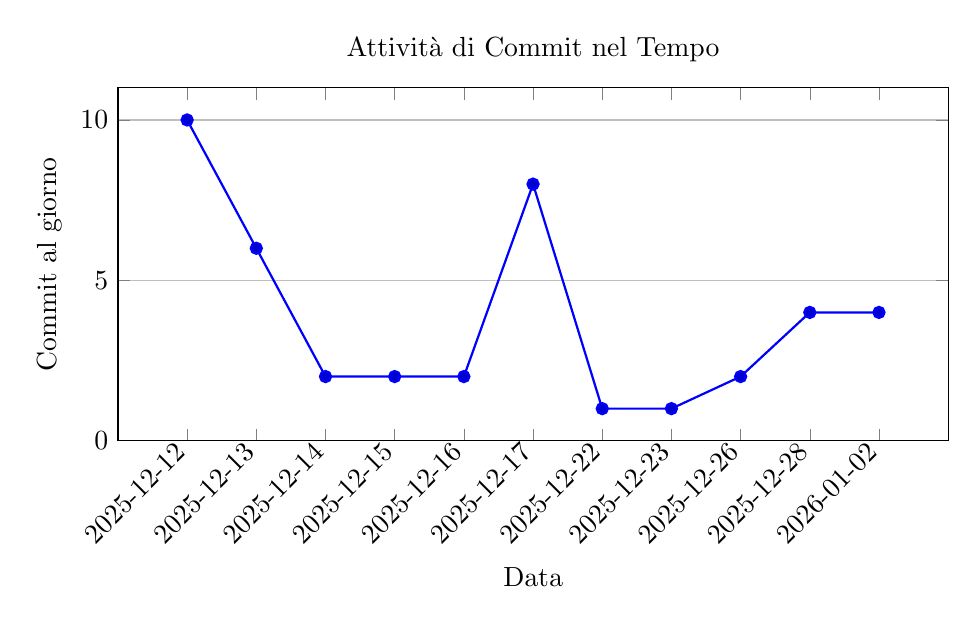
\begin{tikzpicture}
		\begin{axis}[
			width=\textwidth,
			height=0.5\textwidth,
			ymajorgrids=true,
			x tick label style={rotate=45, anchor=east},
			xlabel={Data},
			ylabel={Commit al giorno},
			title={Attività di Commit nel Tempo},
			ymin=0,
			symbolic x coords={2025-12-12,2025-12-13,2025-12-14,2025-12-15,2025-12-16,2025-12-17,2025-12-22,2025-12-23,2025-12-26,2025-12-28,2026-01-02},
			xtick=data
		]
			% Valori derivati da statistiche dei commit del repository
			\addplot+[mark=*, thick, color=blue]
				coordinates {
					(2025-12-12,10)
					(2025-12-13,6)
					(2025-12-14,2)
					(2025-12-15,2)
					(2025-12-16,2)
					(2025-12-17,8)
					(2025-12-22,1)
					(2025-12-23,1)
					(2025-12-26,2)
					(2025-12-28,4)
					(2026-01-02,4)
				};
		\end{axis}
	\end{tikzpicture}
	\caption{Attività dei commit nel tempo (conteggi giornalieri).}
\end{figure}

\section{Report di qualità del codice}
L'analisi statica condotta con SonarQube ha guidato le scelte di qualità durante lo sviluppo.
Per questo progetto ci siamo consapevolmente accontentati di una \textbf{code coverage del 10\%},
privilegiando la consegna delle funzionalità principali. La duplicazione del codice è
\textbf{molto bassa (0.5\%)} su circa \textbf{4000} linee di codice, segno di buona
strutturazione e riuso.

Di seguito è riportato un estratto del report di SonarQube.
\begin{center}
    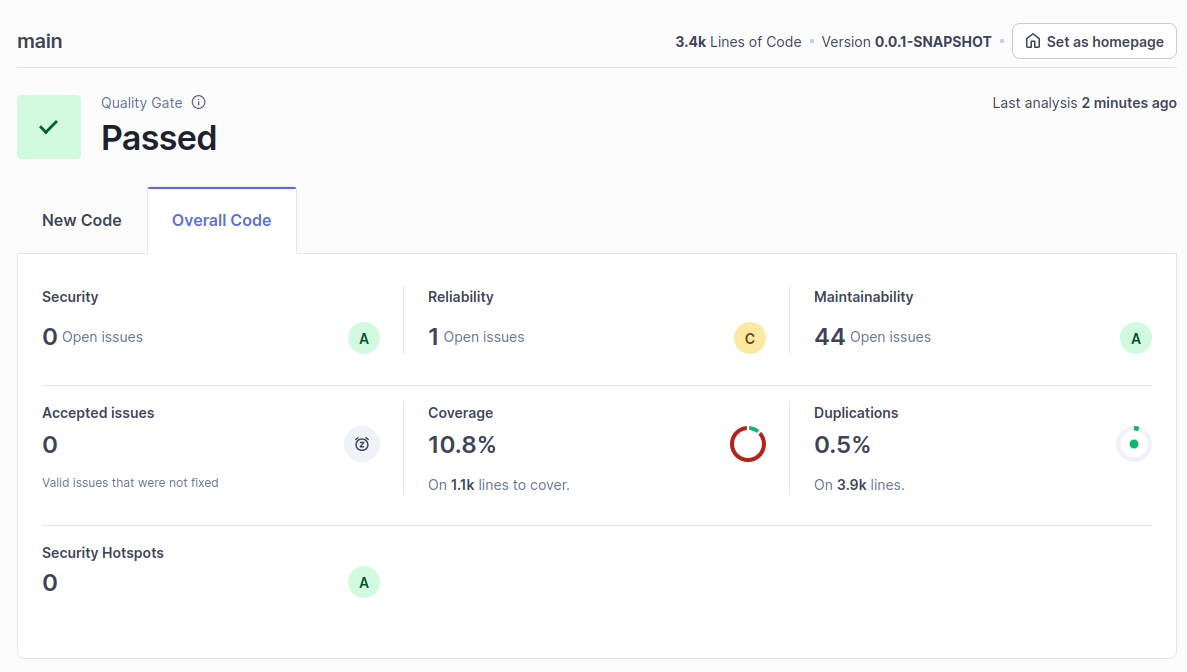
\includegraphics[width=0.8\textwidth]{res/Sonar_Report.png}
\end{center}